\chapter{Introduction}

\section {Motivation}

Single core performance in CPUs has stalled for the last 10 years as processor manufacturers focus on multi-core systems in order to increase performance \cite{procspeed2}. Unfortunately, most of the existing software can not take advantage of the increasing processing speed, because they operate sequentially. Since replacing hardware will not have as much of an impact as it had in the past \cite{procspeed}, scaling legacy systems to modern requirements becomes a very difficult task.

Parallelizing existing software is a daunting proposition as software architectures have a purely sequential design. The programmers involved need to identify parts of their application that consume the most processing time and decide whether it is actually possible to parallelize them. This thesis presents two tools to aid in such attempts.

This thesis presents a framework with two tools developed using Intel Pin \cite{pin} that use dynamic binary instrumentation to obtain information about a application. In order to utilize this data multiple visualizations were developed that help the user in determining which parts of an application can be parallelized. The framework can be easily extended to gather more information that can be displayed in new specialized visualizations.

The framework is based on the concept of tagging sections of a programs source code. This is done interactively and is applied dynamically to the program being instrumented. Changes to the source code of the applications are not required for this tool to function. This makes instrumenting a painless process on complex systems or when dealing with convoluted build processes.

In order to illustrate the usefulness of tools in the analysis of existing software we will present a simple example program in Figure \ref{cap1:emsim:seq}, which needs to be parallelized. The file is part of a simulator for the UEFA European Championship that was implemented sequentially.

\begin{figure}
	\begin{center}
		\inputminted[linenos, fontsize=\scriptsize]{c}{emsim_seq.c}
	\end{center}
	\caption{EM Simulator sequential implementation}
	\label{cap1:emsim:seq}
\end{figure}

By using a profiling tool, the user has determined that the loops present in this code take up almost all the execution time as can be seen in Figure \ref{cap1:emsim:profile} and loops in general have a high potential for parallelism. Now he must determine if their iterations can be run in parallel by examining dependencies between iterations. Intuitively no such knowledge can be gained as a thorough understanding of the application and careful analysis of the loops is required. The pointer arithmetic present in the loop starting in line 12 makes source code inspection very challenging, without understanding the logic behind the implementation it becomes impossible.

\begin{figure}[!ht]
	\centering
	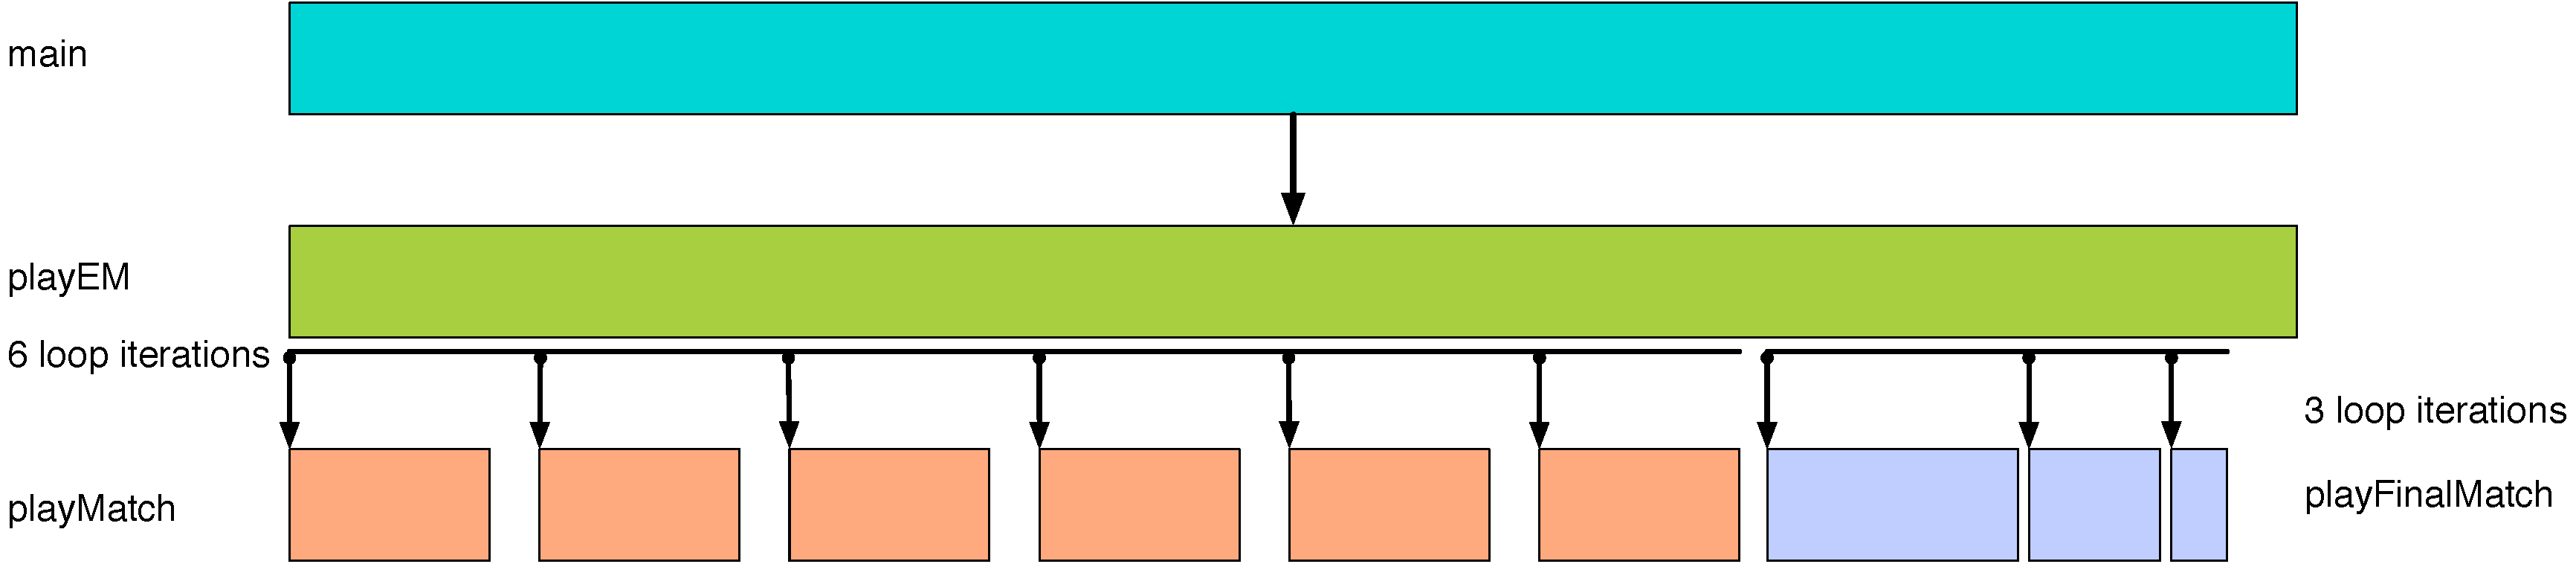
\includegraphics[width=0.8\textwidth]{emsimprofile}
	\caption{Profile view of the execution the code using Parceive}
	\label{cap1:emsim:profile}
\end{figure}

One of our visualizations is able to simulate the speed up when running sections of code in parallel to each other and to show the memory dependencies between the sections. Visualizations of loops on lines 12 and 30 in Figures \ref{cap1:emsim:sections1} and \ref{cap1:emsim:sections2} respectively show the possible speedup when running on a machine with 4 threads and more importantly the actual conflicts that the user must resolve in order to maintain correctness. The loop on line 12 can be easily modified to run in separate threads, even though all iterations work on the same arrays, since each works on distinct elements.

\begin{figure}[!ht]
	\centering
	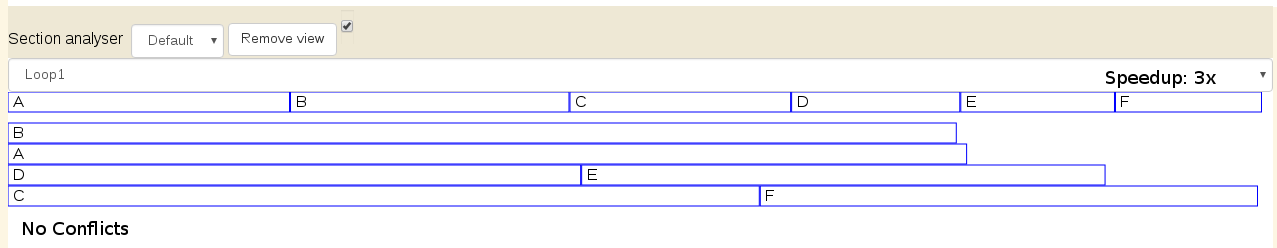
\includegraphics[width=0.8\textwidth]{loop1section}
	\caption{Section view of the loop on line 12 in Figure \ref{cap1:emsim:seq}}
	\label{cap1:emsim:sections1}
\end{figure}

\begin{figure}[!ht]
	\centering
	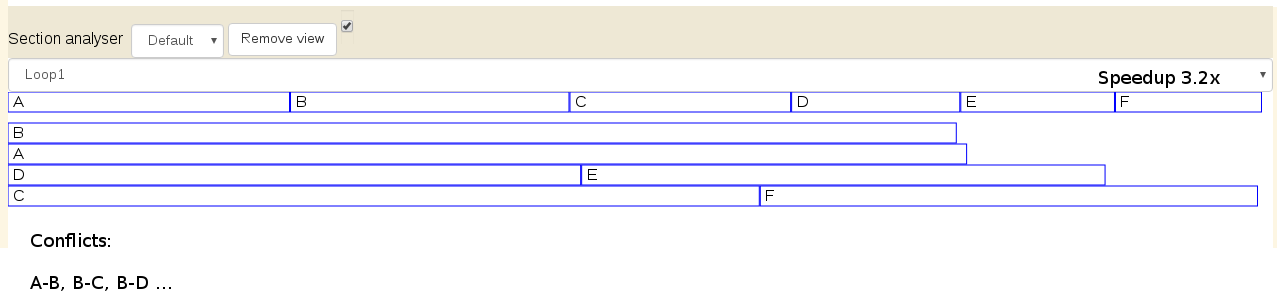
\includegraphics[width=0.8\textwidth]{loop2section}
	\caption{Section view of the loop on line 30 in Figure \ref{cap1:emsim:seq}}
	\label{cap1:emsim:sections2}
\end{figure}

As can be seen in these example, information about the program can be gained by automated tools. Profiling is a well known method of finding performance hot-spots in applications. In this thesis we propose tools that can help determine the potential for parallelization of these sections of code by simulating their parallel execution. This gives the user information about the possible speedup and the problems that require the code to remain sequential.

\section {Contribution}

This thesis presents a framework for gathering information about applications using dynamic binary instrumentation and tagging of the source code. Two use cases have been developed to help users when parallelizing existing applications, but more can be easily developed.

The first use case is a simple analysis that simulates running parts of the source code in parallel. In Figures \ref{cap1:emsim:sections1} and \ref{cap1:emsim:sections2} the loops are tagged as sections and each iteration starts a new task. The visualization presents the possible performance benefit and conflicts when running the tasks within a section in parallel.

Our framework can also perform pipeline analysis to cover a different use case. Pipeline parallelism can be sometimes be applied to loops, despite the fact that iterations can not be run in parallel to each other. This approach splits each iteration into stages and different stages from different iterations can be run parallel to each other. As a simple example we consider file processing, where data is read, processed and written to another file. Individual iterations can not be run in parallel, but the io operations and the processing can be seen in Figure \ref{cap1:pipeline}. In Chapter §2 we will present a more concrete example, bzip compression.

\begin{figure}[!ht]
	\centering
	\begin{tabular}{ l | l | l | l | l}
		R & P & W & & \\
		\hline
		R &  & P & W & \\
		\hline
		R &  & & P & W \\
	\end{tabular}
	\caption{Pipeline, R - read, P - proecess, W - write}
	\label{cap1:pipeline}
\end{figure}

\section {Related Work}

\subsection{Profiling and Tracing}

The tools presented in this thesis are able to gather tracing information about the application, but it is imprecise and slow in this regard. As such it is recommended to use an existing profiler or tracer to discover the performance bottlenecks. Our framework becomes useful after this step, as it helps the user to determine how to eliminate the bottlenecks.

\subsection{Parceive}

Parceive \cite{parceive} is a tracing-based tool for parallelizing existing sequential software. It focuses on high-level architecture analysis, but also gathers fine-grained memory accesses and call information.

The implementation of this tool generates a database compatible with Parceive, keeping all of its existing views functional. The biggest difference is that additional information about tags is recorded, making our analysis possible. The tracing can also be controlled using tags, making it possible for large applications to be analyzed.

We have also created multiple new views that are designed to help a developer in analyzing parallelization opportunities. These visualizations are based on the framework provided by the Parceive UI.

\subsection{Intel Advisor}

Intel Advisor \cite{inteladvisor} is a collection of related tools that focus on helping developers parallelize applications to take advantage of modern processors. It focuses on vectorization and thread parallelism.

The section analysis that this framework provides is also possible in Intel Advisor, but with a different workflow. The source code of the application needs to be annotated using macros provided by the tool such as \texttt{ANNOTATE\_SITE\_BEGIN} or \texttt{ANNOTATE\_TASK\_BEGIN}. This requires rebuilding the application and then instrumenting it using Intel Pin. Our tool is able to instrument the application without the need for source code changes, reducing the number of steps required to gain information about the application.

Intel Advisor also offers many features not available in our tool such as vectorization and memory access pattern analysis. We expect the two tools to complement each other when trying to achieve the greatest performance gains.

\section {Outline}